\documentclass[twoside,10.5pt]{article}
\usepackage{jmlr2e}
%\usepackage{multicol}
%\usepackage[landscape]{geometry}
\usepackage{subfigure}
\usepackage{hyperref}
\usepackage{endnotes}
\usepackage{enumitem}
\let\footnote=\endnote
\renewcommand{\notesname}{Endnotes}
\newcommand{\dataset}{{\cal D}}
\newcommand{\fracpartial}[2]{\frac{\partial #1}{\partial  #2}}
\ShortHeadings{95-845: AAMLP Proposal}{Gangwar, Rost and Setia}
\firstpageno{1}

\begin{document}

\title{Heinz 95-845: Project Report}

\author{\name Mridul Gangwar \email mgangwar@andrew.cmu.edu \\
       \addr Heinz College of Information Systems and Public Policy\\
       Carnegie Mellon University, Pittsburgh, PA, United States \
       \AND
       \name Lauren Rost \email lrost@andrew.cmu.edu \\
       \addr Heinz College of Information Systems and Public Policy\\
       Carnegie Mellon University, Pittsburgh, PA, United States \
       \AND
       \name Nikita Setia \email nikitas@andrew.cmu.edu \\
       \addr Heinz College of Information Systems and Public Policy\\
       Carnegie Mellon University, Pittsburgh, PA, United States}
       
\maketitle
%\begin{multicols}{2}
%\section{Project Details} \label{details}

\begin{abstract}
Opioid overdose deaths spiked in 2017, continuing to be a major concern for the US healthcare system. Major efforts have been dedicated to understand the demographic impacted and how the healthcare system can improve outcomes for individuals at risk. This paper explores the application of machine learning and statistical analyses to identify which could best predict (and prevent) overdose deaths using county-provided demographic, program activity and opiate prescription fills data for Medicaid beneficiaries from 2009-2017. The most superior models, Logistic Regression and Random Forest, yield an AUROC of approximately 85\%, correctly identifying 57\% of individuals who overdose. *Need to add a line about variable importance*. As such, this paper showcases how county-provided data can be used to predict and prevent overdoses (translatable to other counties), identifies the variables indicative of risk, and highlights modeling techniques that can be tuned to improve predictive performance, thereby taking a giant step towards overdose prevention.  
\end{abstract}

%\vspace*{5px}
\section{Introduction}
Opioid abuse has been an emerging public health issue, and was declared a Public Health Emergency in 2017\footnote{\cite{HHS}}. National drug overdose deaths have increased over the past two decades, from 16,849 in 1999 to 70,237 in 2017\footnote{\cite{NIDA_ODR}}. This trend is especially affected by the onset of the opioid epidemic in the late 1990s\footnote{\cite{NIDA_OOC}}. Approximately 67\% of the overdose deaths in 2017 are due to involvement of any opioids and 24\% are specifically due to prescription opioids \footnote{\cite{NIDA_ODR}}. As such, it has become pertinent, now more than ever before, to better understand the risk factors leading to overdoses and to determine the best way to prevent overdose deaths. \\

Crosier et al. predicted overdose frequency using random forests in order to uncover important features related to overdose frequency and course\footnote{\cite{Sage}}. Lobo et al. identified sub-groups of Pennsylvania patients at greater risk for opioid abuse in a k-means clustering algorithm\footnote{\cite{Lobo}}. This paper aims to contribute to this existing body of work by identifying data variables that are most indicative of risk, which could be crucial to preventing addiction and overdoses. \\

In 2005, the Opioid Risk Tool was developed to help flag patients at risk for opioid abuse and overdose\footnote{\cite{Webster}}. However, due to the subjective nature of this tool and the spike of deaths in 2017, machine learning has been sought to provide a more objective and quantitative approach to estimate risk of opioid abuse and overdose. Acion et al. used a super learning approach to predict the successful treatment for patients with substance use disorders\footnote{\cite{Acion}}. Haller et al. utilized natural language processing on electronic health record data to assess risk and predict opioid abuse \footnote{\cite{Haller}}. \\

This paper strives to expand upon the aforementioned previous work, by identifying the machine learning algorithms that yield the highest predictive performance. Specifically, those models that correctly identify the greatest number of at-risk individuals. 

\section{Background}
This project uses a set of demographic features, usage of county-provided programs, and opioid prescription information to predict overdose deaths (opioid and non-opioid). Specifically, it analyzes the data of Medicaid beneficiaries from 2009 to 2017 provided by Allegheny County Department of Human Services (DHS) to predict the risk of an individual dying due to an non-opioid or opioid-related overdose. The likely outcome of this analysis is the finding of at least one feature and at least one machine learning technique that is highly deterministic in the prediction of overdose deaths, thereby enhancing the space of addiction and overdose death prevention. 

\section{Methods}
\subsection{Original Data Description}
DHS provided 3 datasets: demographic, program activity, and opiate prescription fills. These provide information for 120,650 individuals who have utilized DHS services between 2009 and 2017. The demographic dataset contains the following variables: person ID, race and gender. Figure \ref{fig:orig_dem} in the appendix displays the summary of the demographic dataset. Two points to note are: first, there are 19,531 individuals with no reported race and 210 individuals with no reported gender; second, there is also only one individual who is transgendered male to female and only 19 individuals who are Native Hawaiian / Pacific Islanders. \\

Figure \ref{fig:orig_prog} in the appendix summarizes the original program activity data. This dataset contains the following variables: person ID, year and month of activity, the relevant activity information, and overdose details, if any. The program-related activity information collected includes: whether CYF program was used as child or parent (binary), the number of criminal court cases (drug or not) filed, whether mental health, drug and alcohol abuse, or prescription service was used (binary), and whether the individual was jailed (binary). Note that if an individual did not overdose, then those variables contained no information for said individual. Else, it was a 0 for non-opiate overdose and 1 for an opiate overdose. As such, this missingness is meaningful. There appears to be no additional missing data in the program activity dataset. \\

Figure \ref{fig:orig_presc} in the appendix showcases the prescription data summary. The prescription information provided includes: the claim number (unique for each row), person ID, age at prescription, dispensed quantity, days supply, fill date, and information specific to the drug (drug strength, name variations, package description, and dosage form). Some points of note are: first, the last two columns (i.e. generic tier description and claim rank) provide no additional information and can be disregarded; second, there are missing, extreme or incomprehensible values in the prescription dataset, such as an age of -7990, dispensed quantity of 17936 and days supply of 907; third, there are three columns containing the drug names which all contain multiple name versions of the same drug; last, there are two columns pertaining to the dosage form, a condensed version and a descriptive version.

\subsection{Data Cleaning and Extraction}
\subsubsection{Demographic Dataset}
The missing race and gender information is possibly missing not at random (MNAR) as it may be directly related to the unreported value itself. So, this missingness was dealt with by allowing it to be its own category. Furthermore, in the race column specifically, given that the "Native Hawaiian / Pacific Islander" category was too small it was merged with the "No Data" category to create a new category called "No Data and Other." This was replicated for the gender column, merging the "Transgendered male to female" and the "No Data" categories into "No Data and Other."  

\subsubsection{Program Activity Dataset}
The program dataset contains 2,402,479 rows as each row is recording the activity (or activities) for an individual in any year-month since they entered the system. Thus, it was crucial to extract meaningful variables at the person ID level regarding each individual's participation in DHS program activities. Here are the cleaning and extraction tasks performed on this dataset:
\begin{enumerate}[topsep=0pt,itemsep=-1ex,partopsep=1ex,parsep=1ex]
  \item Cleaned the outcome variable by converting the 0, 1 and NA to "Non-Opiate Overdose", "Opiate Overdose" and "No Overdose". Then, extracted this information for each individual ($od\_type$) along with the year ($od\_year$), month ($od\_month$) and date ($od\_date$) in case of overdose.
  \item Created new variables summing each individual's program activity usage as follows: usage of CYF program as child ($total\_cyfchild$) and as parent ($total\_cyfparent$), use of mental health, drug and alcohol abuse and prescription services ($total\_mh$, $total\_da$, $total\_rx$), number of months spent in jail ($total\_acj$), and number of criminal cases ($total\_cr\_cases$) and drug-related cases filed in court ($total\_cr\_drug\_cases$) 
\end{enumerate}

\subsubsection{Opiate Prescription Fills Dataset}
This dataset contains 1,161,650 rows as each row is a prescription fill for an individual. Here too, it was crucial to extract viable variables at the person ID level regarding each individual's opiate prescriptions. Here are the cleaning and extraction tasks performed on this dataset:
\begin{enumerate}[topsep=0pt,itemsep=-1ex,partopsep=1ex,parsep=1ex]
  \item 
  \item 
\end{enumerate}

\subsubsection{Final Dataset}

\subsection{Feature Choices}
In a few columns, we had categories with a few values (less than 0.2\%). For the prediction task, we decided to combine such groups to create a separate “Other” category.We also performed a correlation analysis to better understand the relationship between numerical variables. During the exploration we found out some interesting relationship like hydrobit count is positively correlated with total Rx, number of prescriptions, and pill count.\\

During our data cleaning phase, we had created three variables related to morphine milligram equivalent (MME), i.e., average MME, median MME, and mode MME.  When we plotted the distribution of all these variables, we found out median MME to be less skewed and approximately normally distributed. We decided to keep only median MME our prediction purpose and remove the other two to avoid multicollinearity.

As the last step, we set up our prediction as Opiate Overdose vs. No Overdose (includes non-Opiate Overdose). We removed columns which are derived from overdose date to avoid leakage in our machine learning models, as overdose date is proxy for our target column.


\subsection{Cohort}
*Table 1
Inclusion and Exclusion criteria 

\begin{table}[h!]
  \begin{center}
    \caption{Demographics of DHS Cohort.}
    \label{tab:table1}
    \begin{tabular}{l|c|r} % <-- Alignments: 1st column left, 2nd middle and 3rd right, with vertical lines in between
      \textbf{Characteristic} & \textbf{N} & \textbf{Percentage (\%)}\\
      \hline
      $Race$ & $ $ & $ $ \\
      White & 56,754 & 47.04\\
      Black/African-American & 40,573 & 33.63\\
      Biracial/Multiracial & 2,118 & 1.75\\
      Asian & 1,216 & 1.00\\
      American Indian/Alaskan Native & 439 & 0.36\\
      No Data and Other & 19,550 & 16.20\\
      \textbf{Total} & \textbf{120,650} & \textbf{100}\\
      \hline
      $Gender$ & $ $ & $ $ \\
      Female & 73,582 & 60.99\\
      Male & 46,857 & 38.84\\
      No Data and Other & 211 & 0.17\\
      \textbf{Total} & \textbf{120,650} & \textbf{100}\\
      $Age (years)$ & $ $ & $ $\\
      0-19 & 27,128 & 22.48\\
      20-39 & 51,883 & 43.00\\
      40-59 & 35,941 &  29.79\\
      60 \& Over & 5,698 &   4.72\\
      \textbf{Total} & \textbf{120,650} & \textbf{100}\\
    \end{tabular}
  \end{center}
\end{table}

\subsection{Models}
Machine learning methods (MLR, regularized MLR, random forest, boosting, gradient boosting, survival analysis)
Cross-validation

\subsection{Evaluation Criteria}
Can talk about oversampling here, maybe?
Also, need to explain AUROC, accuracy and other criteria we used to evaluate.
Need to note that will also be striving to purely understand probability of survival and see if varies across subgroups (race, gender). Also, will be looking at importance of variables across models (rf, lr, survival). These are not necessarily evaluating these models, but allowing us to compare them and noting them for future work to compare as well. 

\section{Results}

\subsection{AUROC}
We ran a series of machine learning methods to predict overdose deaths. We were not able to detect sufficient overdose deaths with logistic regression, and thus we implemented an oversampling method, Synthetic Minority Oversampling Technique (SMOTE). This gave us a AUC of 0.85. 
We ran multivariate logistic regression on selected features using 5-fold cross-validation.
We then ran ridge regression using lasso regularization and 10-fold cross-validation.
We also applied random forest to predict overdose death, also using 10-fold cross-validation. 
Gradient boosting machine with 10-fold cross-validation led to an AUC of 0.85.
AdaBoost gave poorer performance than the aforementioned methods, with an AUC of 0.75. We then tested the performance of a neural network to predict opioid death, and found an even lower AUC of 0.5, equal to chance. 

\begin{figure}[htp]
\centering
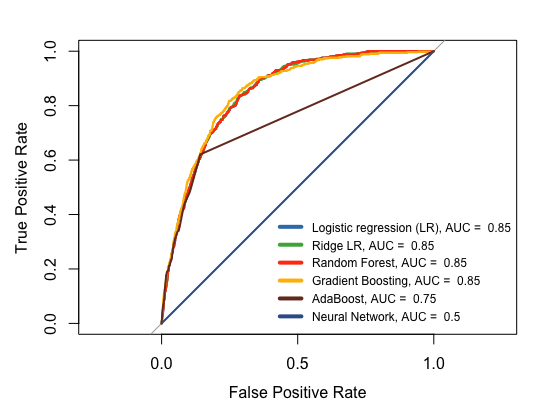
\includegraphics[width=12cm]{images/AUC_ML_opioids.png}
\caption{Predictive performance for overdose deaths had an AUC of 0.85 for three machine learning methods (logistic regression, ridge logistic regression, and random forest), but demonstrated poor performance for gradient boosting, AdaBoost, and neural network).}
\label{fig:lion}
\end{figure}

\subsection{Sensitivity vs. Specificity}

\subsection{Survival Analysis}

\subsection{Variable Importance}


\begin{figure}[htp]
\centering
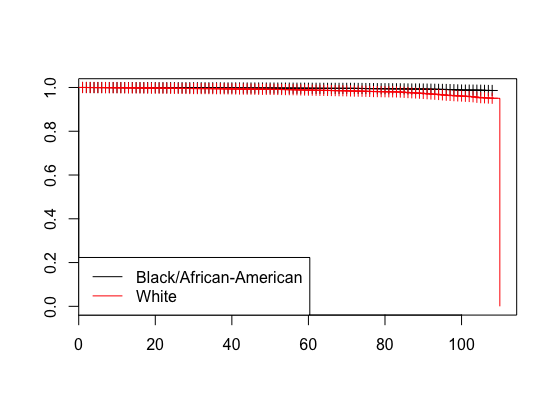
\includegraphics[width=12cm]{images/Race_KaplanMeier.png}
\caption{Kaplan Meier curve of survival indicates that }
\label{fig:lion}
\end{figure}

\begin{figure}[htp]
\centering
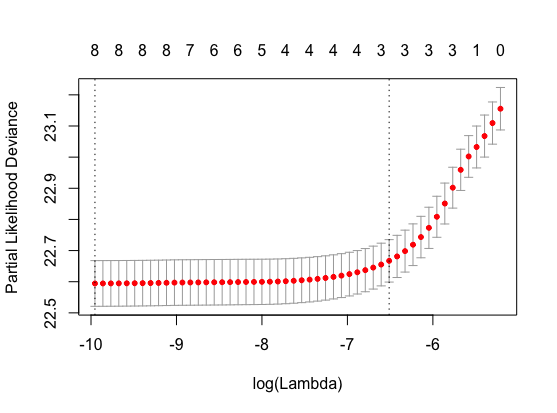
\includegraphics[width=12cm]{images/Coxmodel.png}
\caption{Cox model indicates}
\label{fig:lion}
\end{figure}

\section{Discussion and Related Work}
Significance of results
Limitations 

\section{Conclusion}

\newpage
\appendix
\section*{Appendix A.}
Some more details about those methods, so we can actually replicate them.


\begin{figure}
\begin{center}
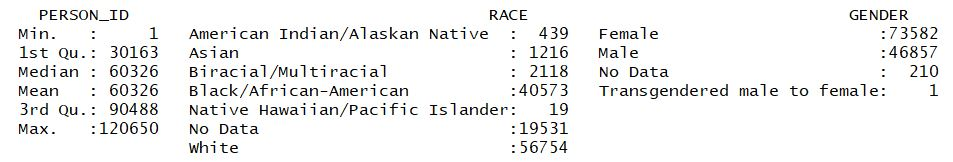
\includegraphics[width=5in]{original_dem_summary.JPG}
\end{center}
\caption{Summary statistics of the original demographic dataset.}
\label{fig:orig_dem}
\end{figure}

\begin{figure}
\begin{center}
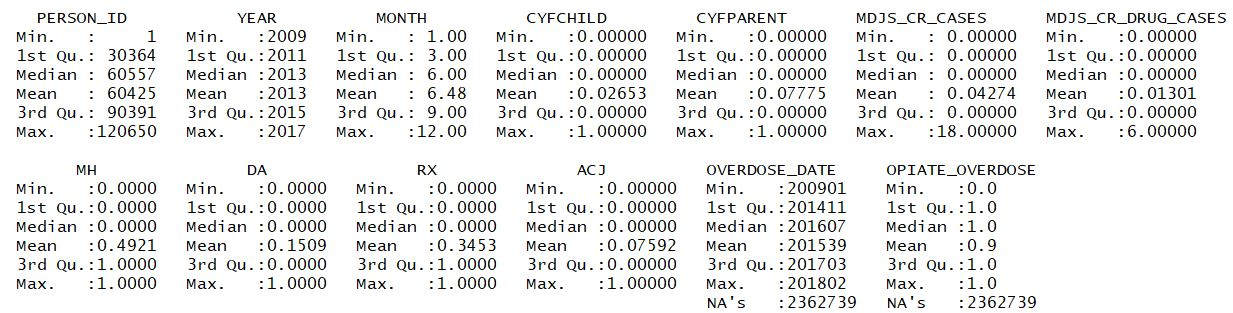
\includegraphics[width=6in]{original_prog_summary.JPG}
\end{center}
\caption{Summary statistics of the original program activity dataset.}
\label{fig:orig_prog}
\end{figure}

\begin{figure}
\begin{center}
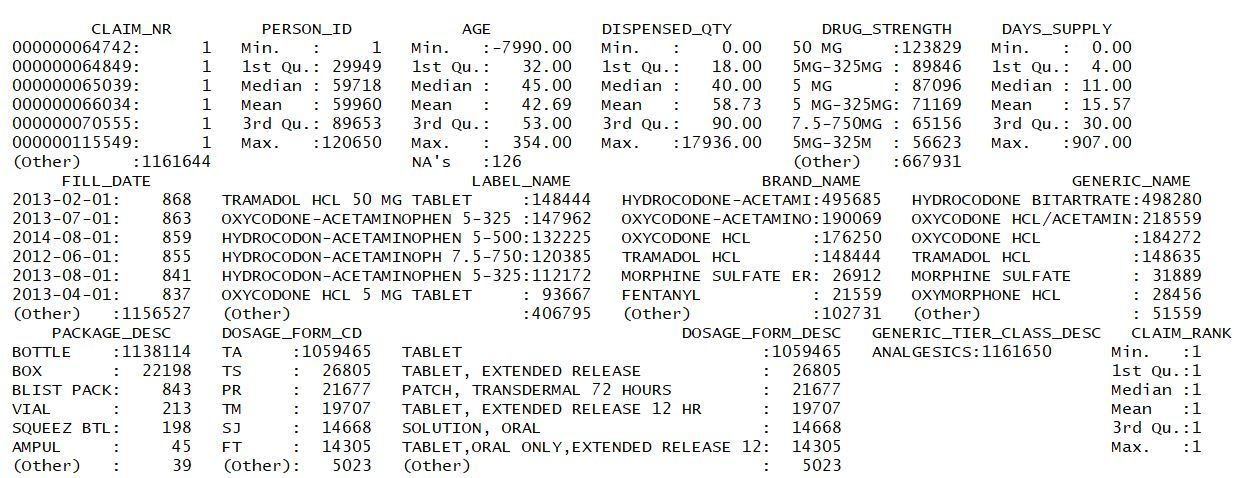
\includegraphics[width=6in]{original_presc_summary.JPG}
\end{center}
\caption{Summary statistics of the original opiate prescription fills dataset.}
\label{fig:orig_presc}
\end{figure}

\newpage
\theendnotes
\bibliographystyle{ieeetr}
\bibliography{final_bibliography.bib}



\end{document} 
